\documentclass[twoside,12pt]{homework}
\newcommand{\n}[1]{\ensuremath{\text{#1}}}
\coursename{COMS W4731 Computer Vision (Fall 2018)} % DON'T CHANGE THIS

\studname{Xingyu Chen}    % YOUR NAME GOES HERE
\studmail{xc2416@columbia.edu}% YOUR UNI GOES HERE
\hwNo{3}                   % THE HOMEWORK NUMBER GOES HERE

% Uncomment the next line if you want to use \includegraphics.
\usepackage{graphicx}

\begin{document}
\maketitle

\section*{Problem 1}

\[\frac{\partial u_{out}}{\partial a} = \frac{\partial(\dfrac{1}{a})}{\partial a} = (a^{-1})^\prime = -\frac{1}{a^2} = -\frac{1}{1.082^2} = -0.854\]
\[\frac{\partial u_{out}}{\partial b} = \frac{\partial u_{out}}{\partial a} \times \frac{\partial a}{\partial b} = -0.854 \times \frac{\partial(b + 1)}{\partial b} = -0.854 \times 1 = -0.854\]
\[\frac{\partial u_{out}}{\partial c} = \frac{\partial u_{out}}{\partial b} \times \frac{\partial b}{\partial c} = -0.854 \times \frac{\partial(e^c)}{\partial c} = -0.854 \times e^{-2.5} = -0.070\]
\[\frac{\partial u_{out}}{\partial d} = \frac{\partial u_{out}}{\partial c} \times \frac{\partial c}{\partial d} = -0.070 \times \frac{\partial(-d)}{\partial d} = -0.070 \times (-1) = 0.070\]
\[\frac{\partial u_{out}}{\partial e} = \frac{\partial u_{out}}{\partial d} \times \frac{\partial d}{\partial e} = 0.070 \times 1 = 0.070\]
\[\frac{\partial u_{out}}{\partial f} = \frac{\partial u_{out}}{\partial e} \times \frac{\partial e}{\partial f} = 0.070 \times 1 = 0.070\]
\[\frac{\partial u_{out}}{\partial g} = \frac{\partial u_{out}}{\partial f} \times \frac{\partial f}{\partial g} = 0.070 \times w_1 = 0.070 \times (-4) = -0.280\]
\[\frac{\partial u_{out}}{\partial h} = \frac{\partial u_{out}}{\partial f} \times \frac{\partial f}{\partial h} = 0.070 \times x_1 = 0.070 \times 1 = 0.070\]
\[\frac{\partial u_{out}}{\partial i} = \frac{\partial u_{out}}{\partial f} \times \frac{\partial f}{\partial i} = 0.070 \times w_2 = 0.070 \times 3 = 0.210\]
\[\frac{\partial u_{out}}{\partial j} = \frac{\partial u_{out}}{\partial f} \times \frac{\partial f}{\partial j} = 0.070 \times x_2 = 0.070 \times 2 = 0.140\]

\newpage
\section*{Problem 2}

See Jupyter Notebook. To run the network, simply run the whole cells of the notebook 'FullyConnectedNets.ipynb'.

\newpage
\section*{Problem 3}

Code see Jupyter Notebook. To run the network for each sub-problem from 3.1 - 3.4, simply run the corresponding notebook file 'problem3\_x.ipynb'. It may take hours to run the network.

\subsection*{1.}

Plots see Figure \ref{fig1} and Figure \ref{fig2}.

\begin{figure}[!htb]
\begin{center}
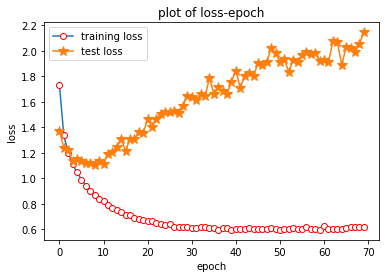
\includegraphics[width=4in]{Unknown-1.png}
\caption{Problem 3.1 Loss Plot}
\label{fig1}
\end{center}
\end{figure}

\begin{figure}[!htb]
\begin{center}
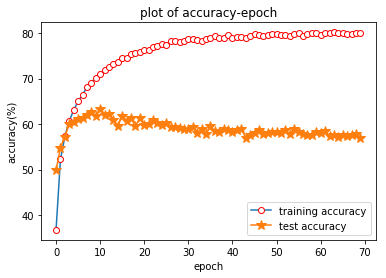
\includegraphics[width=4in]{Unknown-2.png}
\caption{Problem 3.1 Accuracy Plot}
\label{fig2}
\end{center}
\end{figure}

\begin{figure}[!htb]
\begin{center}
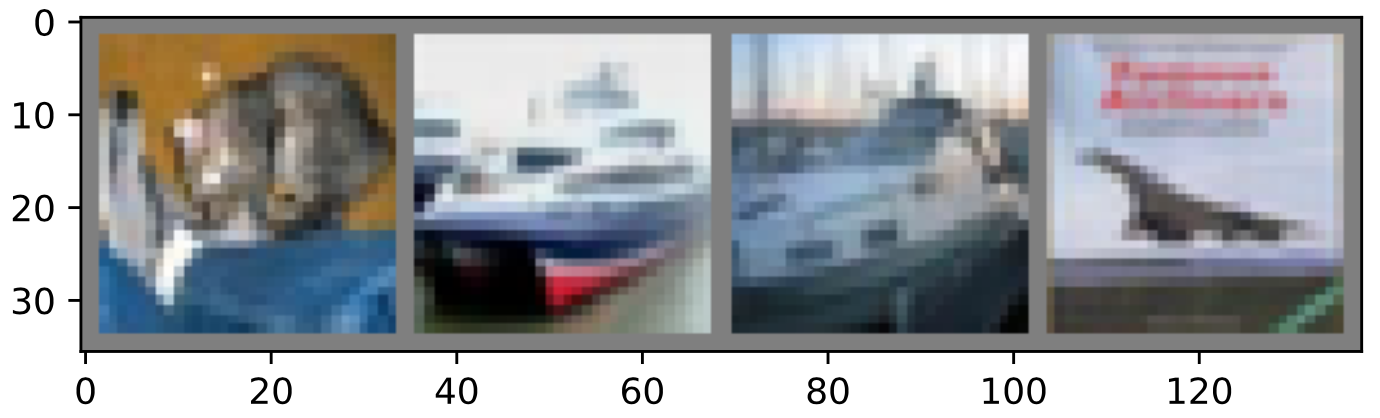
\includegraphics[width=4in]{00.png}
\caption{Predicted Labels: cat ship ship plane, Ground Truth: cat ship ship plane}
\label{fig3}
\end{center}
\end{figure}

\begin{figure}[!htb]
\begin{center}
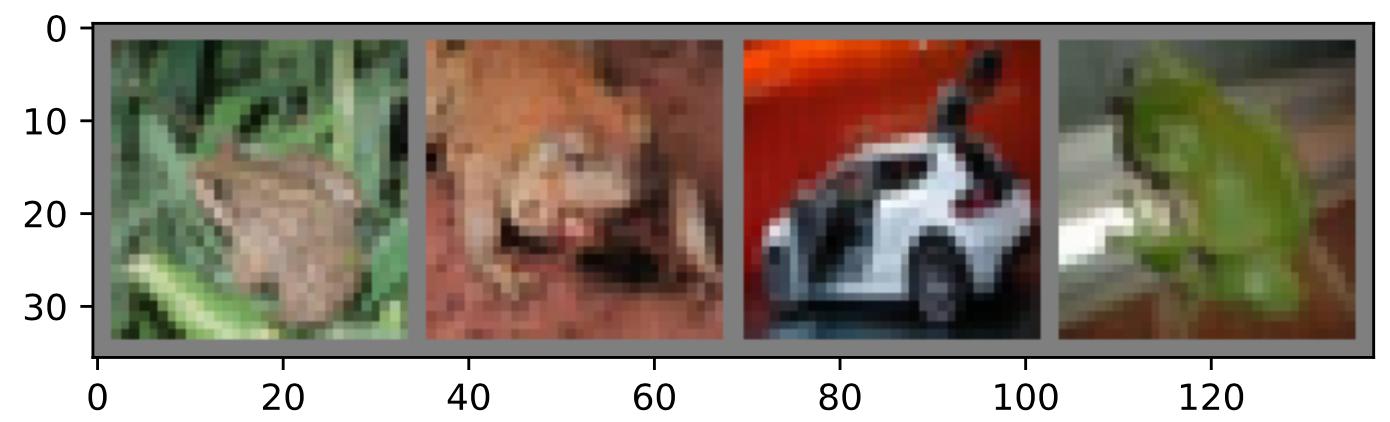
\includegraphics[width=4in]{01.png}
\caption{Predicted Labels: cat frog frog frog, Ground Truth: frog frog car frog}
\label{fig4}
\end{center}
\end{figure}

\begin{figure}[!htb]
\begin{center}
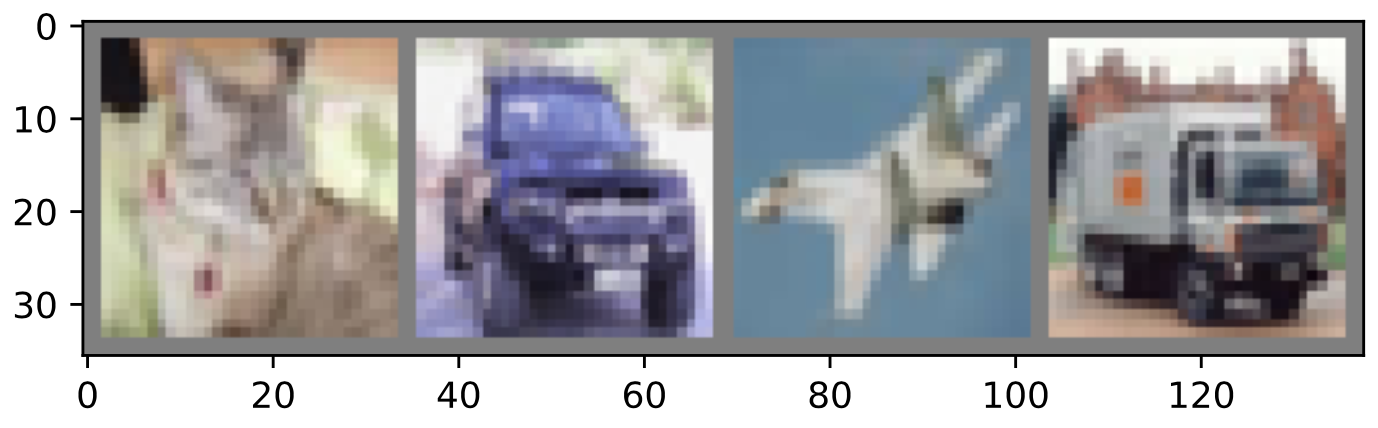
\includegraphics[width=4in]{02.png}
\caption{Predicted Labels: cat car deer truck, Ground Truth: cat car plane truck}
\label{fig5}
\end{center}
\end{figure}

\subsection*{2.}

Plots see Figure \ref{fig6} and Figure \ref{fig7}.

\begin{figure}[!htb]
\begin{center}
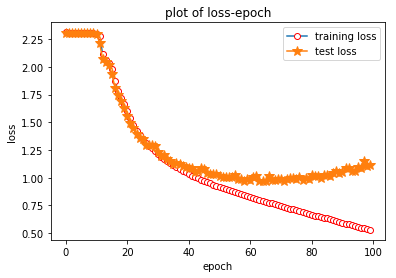
\includegraphics[width=4in]{Unknown-3.png}
\caption{Problem 3.2 Loss Plot}
\label{fig6}
\end{center}
\end{figure}

\begin{figure}[!htb]
\begin{center}
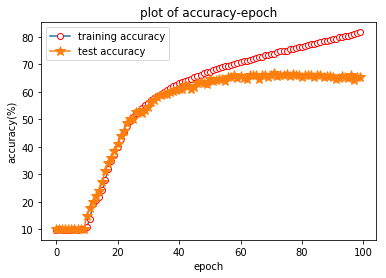
\includegraphics[width=4in]{Unknown-4.png}
\caption{Problem 3.2 Accuracy Plot}
\label{fig7}
\end{center}
\end{figure}

\subsection*{3.}

Plots see Figure \ref{fig8} and Figure \ref{fig9}.\\

\begin{figure}[!htb]
\begin{center}
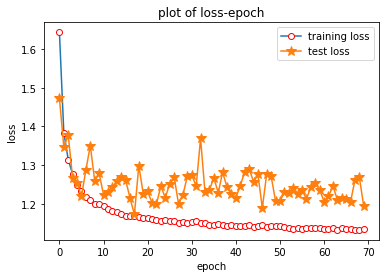
\includegraphics[width=4in]{Unknown-5.png}
\caption{Problem 3.3 Loss Plot}
\label{fig8}
\end{center}
\end{figure}

\begin{figure}[!htb]
\begin{center}
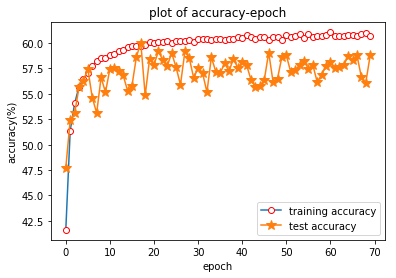
\includegraphics[width=4in]{Unknown-6.png}
\caption{Problem 3.3 Accuracy Plot}
\label{fig9}
\end{center}
\end{figure}

\noindent The performance is changed because the ReLU makes the model non-linear compared to the original one. It can remove the negative activation to zero.

\subsection*{4.}

Plots see Figure \ref{fig10} and Figure \ref{fig11}.

\begin{figure}[!htb]
\begin{center}
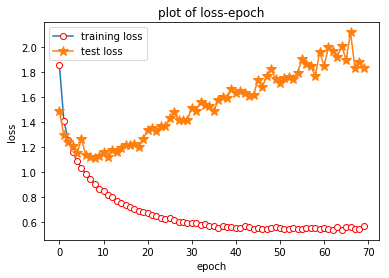
\includegraphics[width=4in]{Unknown-7.png}
\caption{Problem 3.4 Loss Plot}
\label{fig10}
\end{center}
\end{figure}

\begin{figure}[!htb]
\begin{center}
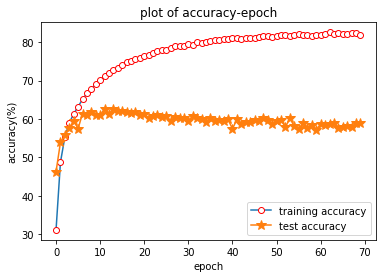
\includegraphics[width=4in]{Unknown-8.png}
\caption{Problem 3.4 Accuracy Plot}
\label{fig11}
\end{center}
\end{figure}

\subsection*{5.}

From the last 4 subsections, I found that 4.2, the sigmoid part, is the best through the test accuracy. For our structure of network, using sigmoid functions the activation function can improve the baseline performance. This is probably because this problem is more suitable to a smooth and non-linear activation function.

\subsection*{6.}

For the first plot, we say the structure of the network is reasonable because both the training the test error is descending and seem to converge to a constant. \\

\noindent For the second plot, we say the model is 'overfit' to the training data because the training error is still descending, indicating that the model is continuously becoming more suitable to the training data. However, after a certain number of epoches, the test error goes up, meaning that the model is too suitable for the training and does poorly on the teat data, which is also general. 

\newpage

\section*{Problem 4}

For the first example, as shown in Figure \ref{fig12}, a frog is mis-labeled as a cat. This is probably because its color and figure are both similar to the general cat type. \\

\begin{figure}[!htb]
\begin{center}
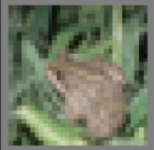
\includegraphics[width=1in]{11.png}
\caption{Predicted Label: cat, Ground Truth: frog}
\label{fig12}
\end{center}
\end{figure}

\noindent For the second example, as shown in Figure \ref{fig13}, a car is mis-labeled as a frog. This is probably because its figure is similar to the general frog type, which is small and round. \\

\begin{figure}[!htb]
\begin{center}
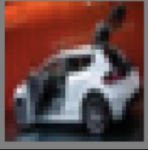
\includegraphics[width=1in]{12.png}
\caption{Predicted Label: frog, Ground Truth: car}
\label{fig13}
\end{center}
\end{figure}

\noindent For the third example, as shown in Figure \ref{fig14}, a plane is mis-labeled as a deer. This is kind of strange because from my raw eyes, I think it is more likely to be mis-labeled as a bird. I think it is probably that all the score for each class is similar and the deer class just has a little advantage.\\

\begin{figure}[!htb]
\begin{center}
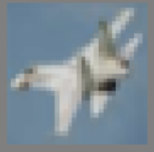
\includegraphics[width=1in]{13.png}
\caption{Predicted Label: deer, Ground Truth: plane}
\label{fig14}
\end{center}
\end{figure}

\noindent For the fourth example, as shown in Figure \ref{fig15}, a frog is mis-labeled as a cat. This is probably because its color and figure are both similar to the general cat type, like the first example.\\

\begin{figure}[!htb]
\begin{center}
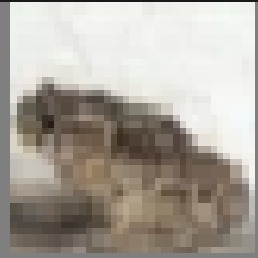
\includegraphics[width=1in]{14.png}
\caption{Predicted Label: cat, Ground Truth: frog}
\label{fig15}
\end{center}
\end{figure}

\noindent For the fifth example, as shown in Figure \ref{fig16}, a bird is mis-labeled as a dog. This is probably because this bird is back to the camera and does not display the specific bird characteristics.

\begin{figure}[!htb]
\begin{center}
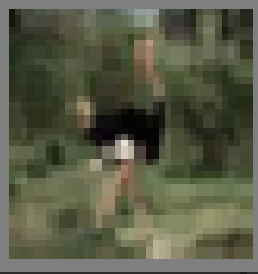
\includegraphics[width=1in]{15.png}
\caption{Predicted Label: dog, Ground Truth: bird}
\label{fig16}
\end{center}
\end{figure}

\end{document} 

